\documentclass[a4paper,12pt]{report}

\usepackage{alltt, fancyvrb, url}
\usepackage{amssymb}
\usepackage{cleveref}
\usepackage{graphicx}
\usepackage{subfigure}
\usepackage{sidecap}
\usepackage{wrapfig}
\usepackage{amsmath,amssymb,stmaryrd,mathtools,alltt}
\usepackage{algorithmic, algorithm}
\usepackage[utf8]{inputenc}
\usepackage{fontenc}
\usepackage{url}
\usepackage{cleveref,amsmath,amssymb,stmaryrd,mathtools,alltt,algorithm}
\usepackage{amssymb}

\usepackage[left=2cm, right=2cm, bottom=3cm]{geometry}

\usepackage[italian]{babel}



\begin{document}
\title{SmarterCities}
 
\author{Federico Bellini \& Francesco Capponi}

\date{\today}
 
\maketitle

\tableofcontents
 
\vfill
\chapter{Analisi}
\section{Introduzione}
\subsection*{L'idea}
L’idea di questo progetto è venuta osservando il sistema stradale di controllo 
e prevenzione che negli Stati esteri sta diventando sempre più presente e 
capillare. Ovviamente tutto questo ha i suoi lati positivi e negativi, a 
seconda del fine che il controllo ha. Il nostro software, denominato 
SmarterCities, si limiterà ad effettuare una dimostrazione pratica di alcune 
azioni che potrebbero esser fatte se potessimo essere in possesso di suddetti 
dati, senza esprimere giudizi etici o morali al riguardo.

\subsection*{Perché è possibile}

\begin{wrapfigure}{r}{0.4\textwidth}
  \vspace{-40pt}
  \begin{center}
      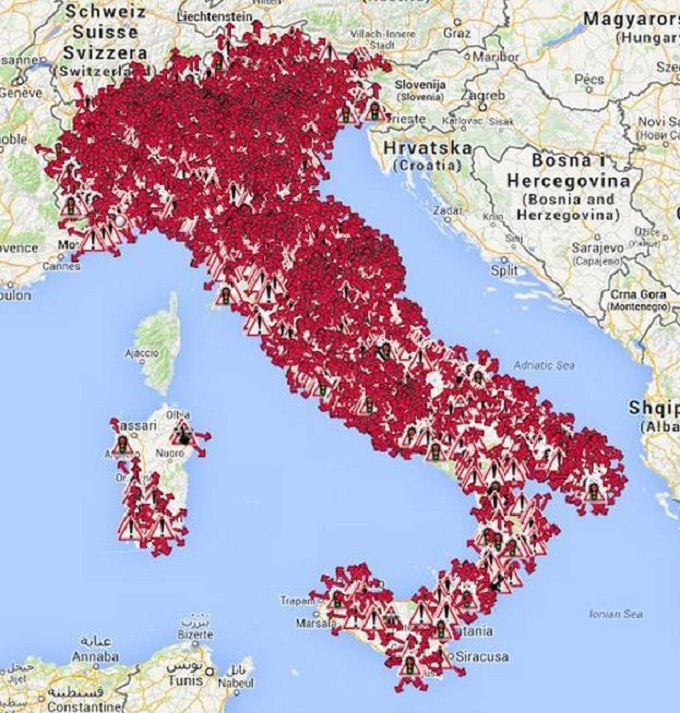
\includegraphics[width=0.38\textwidth]{images/mappaAutoveloxItalia}
    \caption{Mappa degli Autovelox in Italia}
    \label{fig:mappaAutoveloxItalia}
  \end{center}
  \vspace{-10pt}
\end{wrapfigure}
E' da tenere in considerazione che in Italia già esiste una fitta rete di 
controllo stradale automatica, composta da autovelox, tutor etc. Questi enti 
distribuiti su tutto il territorio generano enormi quantità di dati 
quotidianamente, che vengono già utilizzati per scopi legislativi e 
regolamentari, ma sono gestiti come singole entità e quindi quasi totalmente 
privi di elaborazione. \newline
Di conseguenza è già idealmente possibile offrire alla comunità il servizio che 
la nostra applicazione propone.

\subsection*{Il risultato desiderato}
Con questa applicazione si potrebbero offrire ad esempio servizi di 
monitoraggio del traffico, analizzando le strade con maggior affluenza di una 
città; calcolare la velocità media realmente rispettata su ogni strada e 
prendere provvedimenti di conseguenza(aggiunta dossi ecc..). In aggiunta con un 
piccolo upgrade si potrebbe offrire un servizio di vigilanza, controllando 
le strade ed avvertendo le autorità quando viene avvistato un mezzo 
rubato.\newline
Lo scopo dell’applicazione è quindi quello di mostrare come si possa creare un 
server che gestisca le informazioni raccolte per le strade dai vari rilevatori 
con fini utili alla comunità.

\section{Funzionalità}

Il software è composto da tre funzionalità principali ed un esempio di 
estensione: dovrà permettere di raccogliere i dati dalle varie fonti, salvare i 
suddetti dati, simulare una situazione pseudo reale di traffico cittadino e 
fornire un esempio di elaborazione dei dati ottenuti.

\subsection{Ricezione dati}
La funzionalità core per una Smart City è proprio quella di porter ricevere i 
dati da più fonti. Per questo è stata implementata una specifica interfaccia 
che consente ai Tutor, Autovelox e simili (che da ora in poi per generalizzare 
chiameremo ``Street Observers`` o ``Osservatori``), di inviare i dati acquisiti 
(denominati ``Sightings``, o ``Avvistamenti``).

\subsection{Salvataggio dati}
Essendo un software finalizzato all'analisi dei dati, è fornita un'interfaccia 
che consente il salvataggio delle informazioni ricevute su una memoria stabile.

\subsection{Simulazione}
Non avendo a disposizione degli Osservatori reali che ci inviano dati, 
ai fini di una dimostrazione pratica, abbiamo implementato un'interfaccia che 
genera dati pseudo-casuali. 

\subsection{Elaborazione}
E' possibile creare infiniti esempi di elaborazione dei dati. Nel nostro
specifico caso abbiamo scelto di creare tre differenti interfacce per 
l'elaborazione delle informazioni:
\begin{itemize}
  \item Una prima interfaccia che consente di ottenere informazioni generali, 
quali la frequenza giornaliera/mensile ecc. di auto avvistate da un 
Osservatore, la velocità media rilevata ed ulteriori parametri ricavati dai 
dati spediti dagli Osservatori.
  \item Una seconda interfaccia che mostra su di una mappa la posizione 
effettiva degli Osservatori;
  \item Una terza interfaccia che verifica ad ogni Avvistamento, che la 
macchina passata non sia stata rubata. Se così fosse dovrà essere segnalata 
questa evenienza all'operatore.
\end{itemize}


\chapter{Design}

\section{Architettura complessiva}

Si nota da subito guardando la figura 
~\ref{fig:smartCitiesTresSimpleDiagram} dello schema generale che segue, 
che l'applicazione ha più di un punto di entrata: Utente e Network. In questa 
situazione pare ovvio usare il pattern \textit{Model-View-Controller}. Così 
facendo infatti, sia la \textit{GUI} che il \textit{Network} sono trattati come 
due differenti \textit{View}. Infatti la \textit{GUI} sarà un'interfaccia View 
per gli ''operatori umani``, mentre il \textit{Network} sarà un'interfaccia per 
gli operatori meccanici, come gli \textit{Street Observers}.
Con questo genere di implementazione possiamo quindi avere conferma della 
corretta implementazione del Controller, dimostrando che esso può gestire più di 
una singola View.\newline
Di conseguenza il Controller sarà punto cardine dell'applicazione, processando 
gli eventi provenienti dalle Views, ed interfacciandosi con il Model, ossia il 
Database contenente tutti i dati ricevuti. 
In particolare visto che il \textit{Network}, ricevendo messaggi da parte degli 
Street Observers, genera a sua volta dei messaggi che andranno ad influire 
sulla \textit{GUI}, il \textit{Controller} si dovrà preoccupare anche di 
sincronizzare le due parti.
\newpage
\section {Schema Generale}
\begin{figure}[H]
  \centering
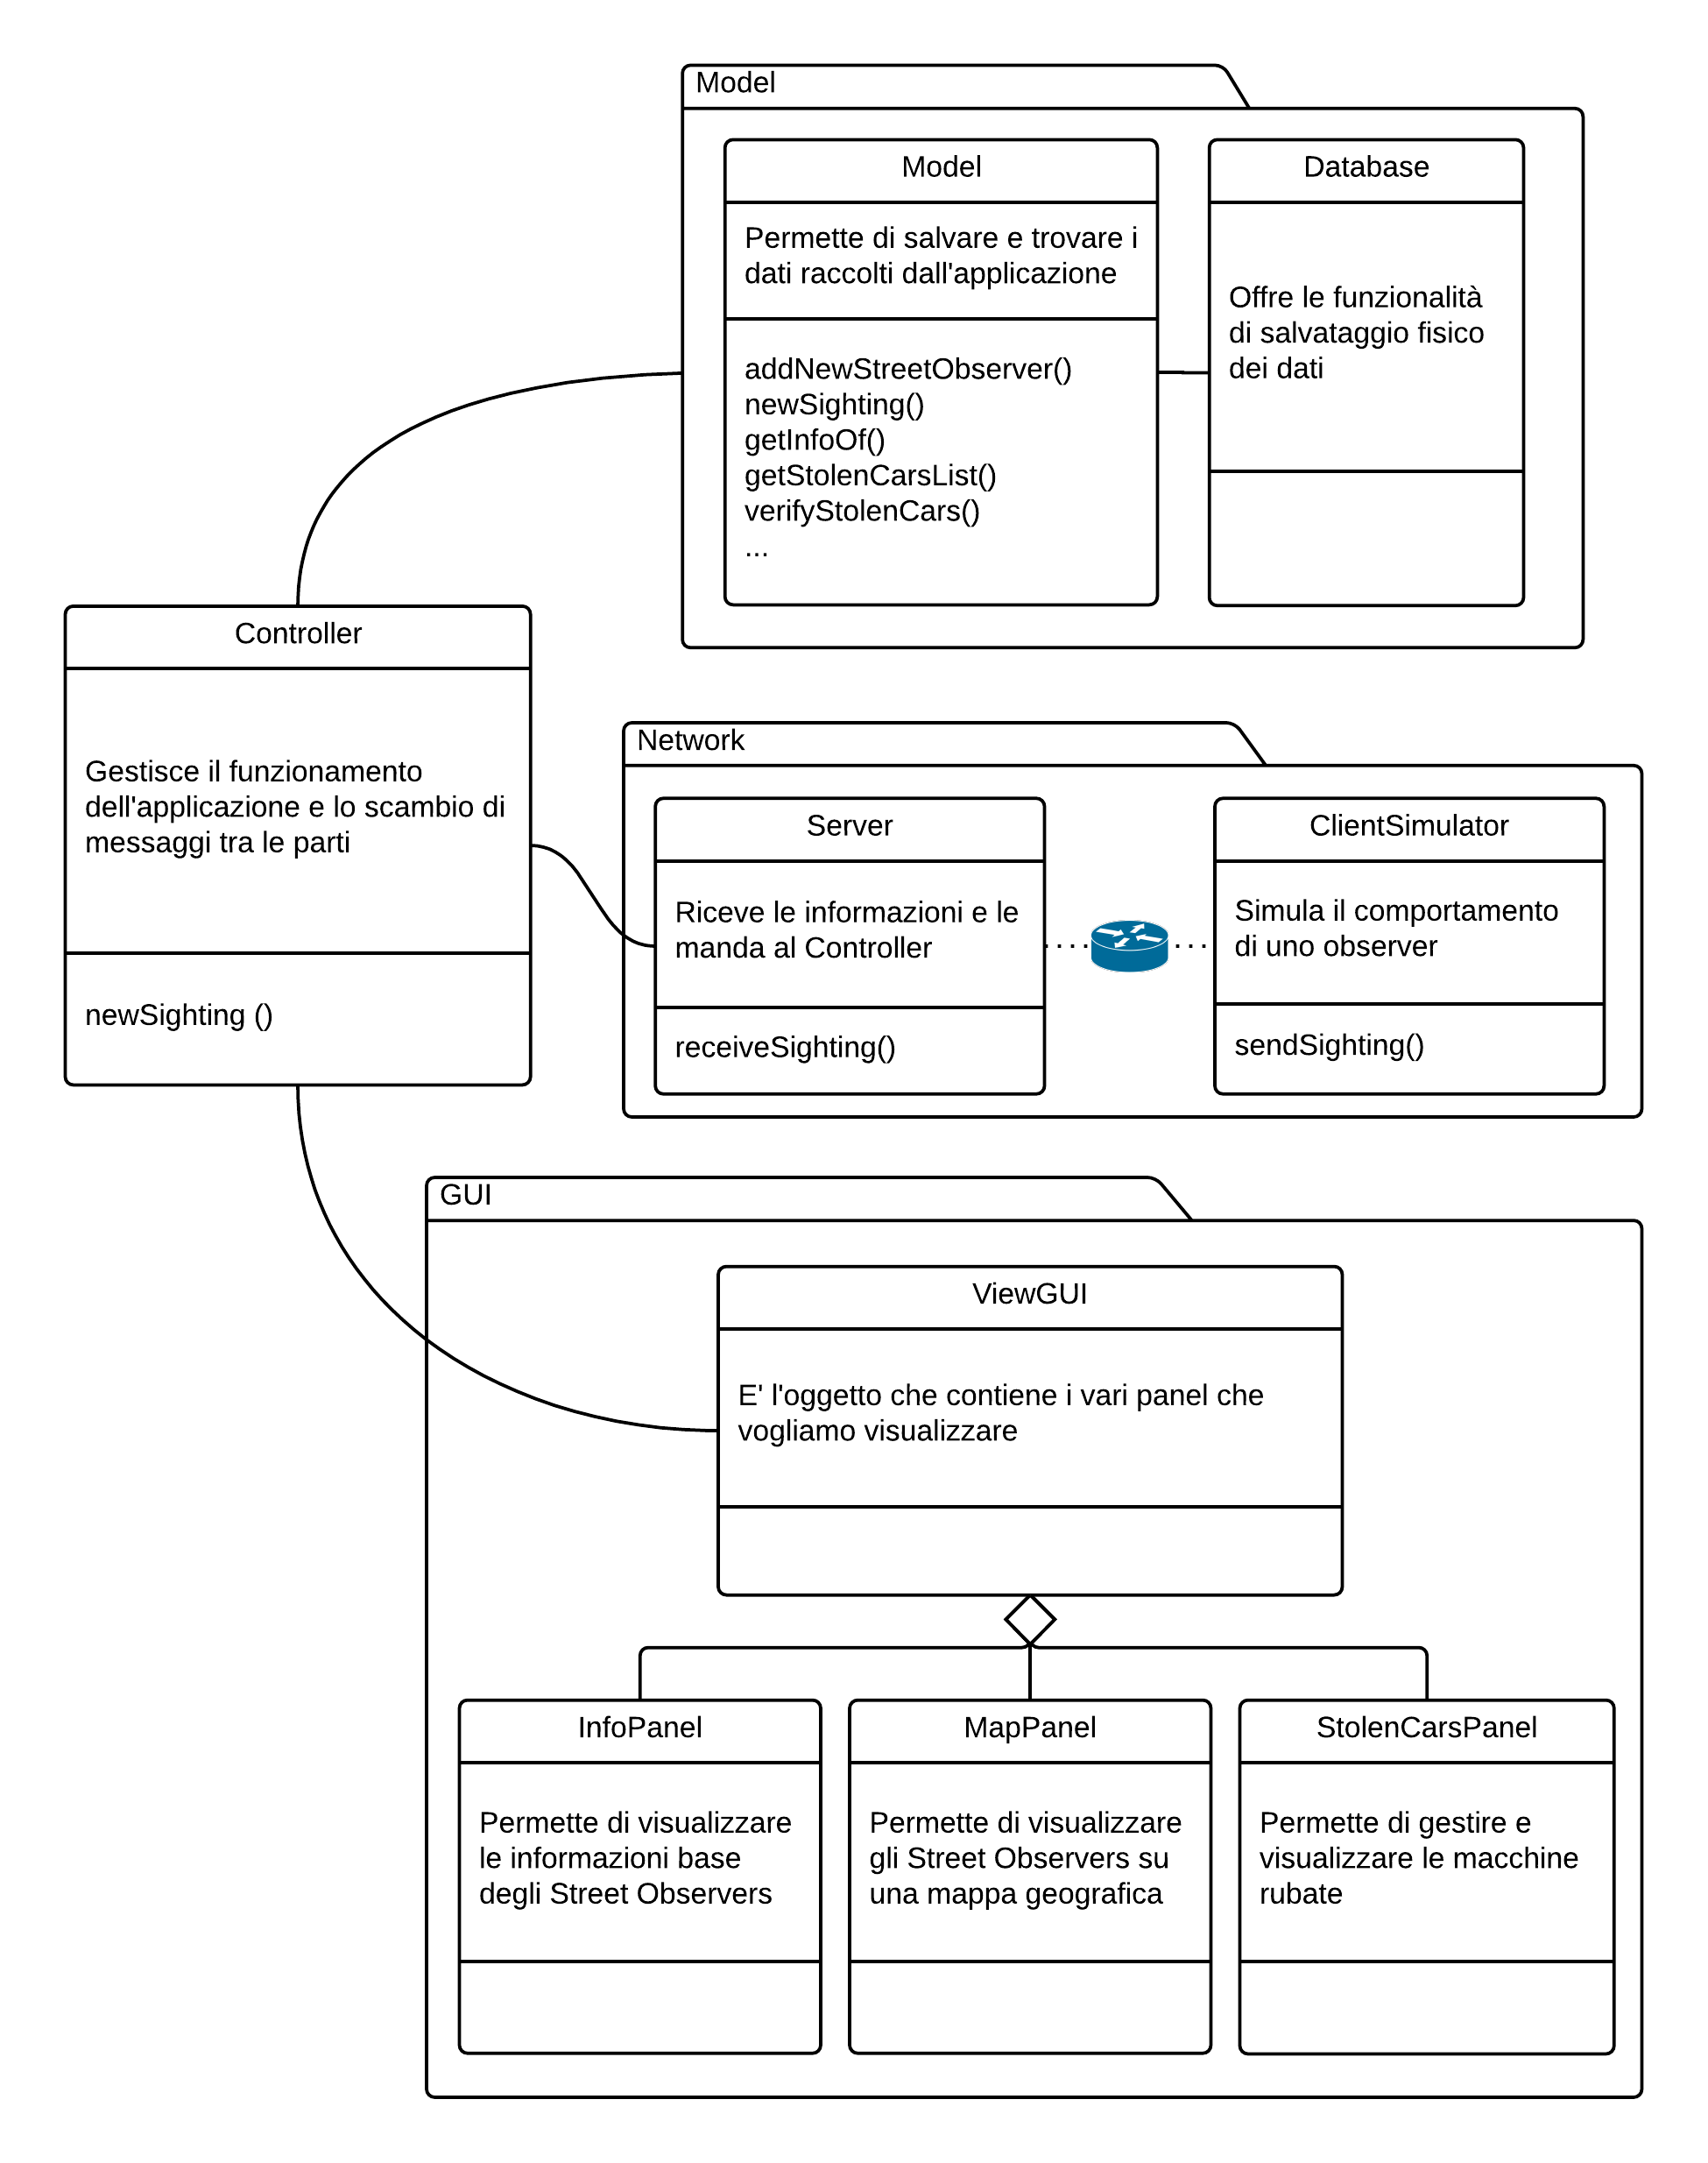
\includegraphics[width=0.90\textwidth]{images/smartCitiesTresSimpleDiagram}
  \caption{Descrizione dell'architettura per macroblocchi}
  \label{fig:smartCitiesTresSimpleDiagram}
\end{figure}
\clearpage
\section{Pattern Utilizzati}

  \subsection{Controller}
    \subsubsection{Decorator}
      \begin{wrapfigure}{r}{0.5\textwidth}
	\vspace{-40pt}
	\begin{center}
  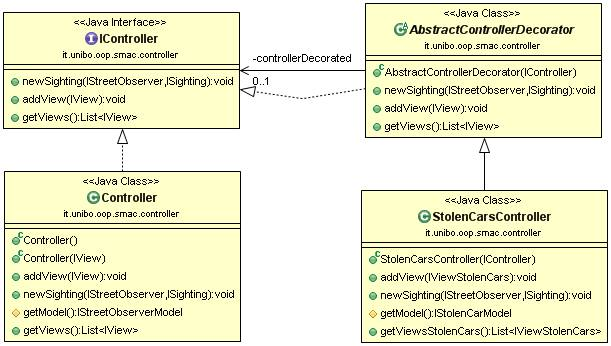
\includegraphics[width=0.48\textwidth]{images/UMLcontroller}
	\caption{UML descrittivo del decorator del Controller}
	\label{fig:UMLcontrollerDecorator}
	\end{center}
	\vspace{-20pt}
      \end{wrapfigure}
      Di default il Controller mette a disposizione solo l'interfaccia per la 
gestione degli Street Observers e dei Sighting.\newline
      Per mostrare le possibilità di future estensioni dell'applicazione, 
abbiamo voluto aggiungere delle funzioni all'\textit{IController} utilizzando 
il pattern \textit{Decorator}, implementato dalla classe     
\textit{AbstractControllerDecorator}. 
    In questo modo tramite l'implementazione dello \textit{StolenCarsController} 
    che decora un \textit{IController}, in un solo Controller siamo in 
grado di gestire anche le funzionalità riguardanti le macchine rubate.

    
    \subsubsection{Observer}
    \begin{wrapfigure}{r}{0.5\textwidth}
      \vspace{-40pt}
      \begin{center}
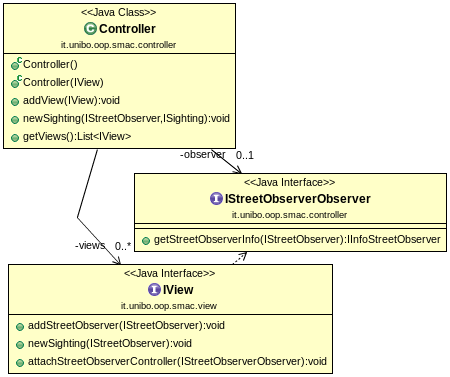
\includegraphics[width=0.48\textwidth]{images/UMLcontrollerObserver}
	\caption{UML descrittivo degli obsever del Controller}
	\label{fig:UMLcontrolerObserver}
      \end{center}
      \vspace{-10pt}
    \end{wrapfigure}
      
      Il Controller, è strettamente legato alle Views, poiché 
deve gestirne gli eventi. Per garantire un maggior indipendenza tra le due 
parti, alla View non è permesso di richiamare direttamente i metodi del 
Controller, ma ogni View scatenerà degli eventi su un'ulteriore classe che ne 
fa da Observer, la quale poi si occuperà di richiamare il giusto metodo del 
Controller per ogni differente evento. In questo modo se in futuro avverrà un 
cambiamento della ai metodi del controller, non causerà la modifica della View, 
che farà riferimento univocamente alla classe Observer 
(\textit{InfoStreetObserverObserver}. 
Le classi a cui vengono \textit{attached} questi Observer sono: 
\textit{IView} (con la funzione attachStreetObserverObserver) e
\textit{IViewStolenCars} (con la funzione attachStolenCarsObserver). Nella 
figura~\ref{fig:UMLcontrolerObserver} abbiamo mostrato soltanto il caso del 
\textit{Controller} e relativa \textit{IView}. Il caso dello 
\textit{StolenCarsController}, è del tutto analogo.
\clearpage
  \subsection{GUI}
    \subsubsection {ViewGUI: Façade}
    \begin{wrapfigure}{r}{0.4\textwidth}
      \vspace{-80pt}
      \begin{center}
	  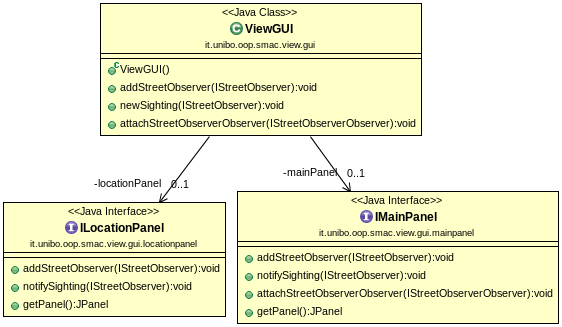
\includegraphics[width=0.38\textwidth]{images/UMLviewFacade}
	\caption{UML descrittivo del facade nella GUI}
	\label{fig:UMLviewFacade}
      \end{center}
      \vspace{-10pt}
    \end{wrapfigure}

     La GUI è composta da una una serie di panel per la gestione della 
visualizzazione delle varie componenti dell'applicazione. Per rendere più 
semplice e leggibile il codice, tutti i panel vengono gestiti da un'unica 
classe, implementata secondo il pattern Façade, che quindi gioca un ruolo di 
'facciata' per tutte le altre, permettendo in questo modo un accesso più 
facile a tutte le sue sottoclassi.

    \subsubsection {AbstractMapMarker: Template Method}
    \begin{wrapfigure}{r}{0.4\textwidth}
      \vspace{-60pt}
      \begin{center}
	  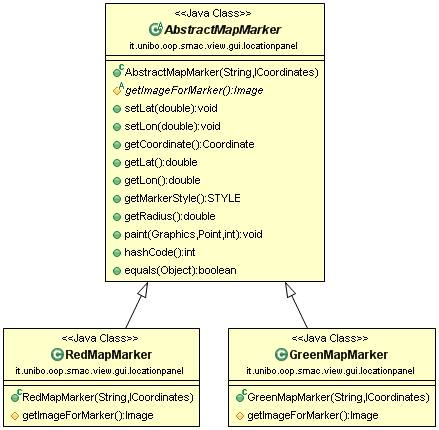
\includegraphics[width=0.38\textwidth]{images/UMLmapMarker}
	\caption{UML descrittivo del Template Method dell'AbstractMapMarker}
	\label{fig:UMLmapMarker}
      \end{center}
      \vspace{-60pt}
    \end{wrapfigure}

    La classe \textit{AbstractMapMarker} implementa un generico 
\textit{MapMarker} (ossia un'icona che deve essere visualizzata su di una mappa 
per marcarne una posizione), lasciando il compito alle classi che la estendono 
di scegliere la specifica icona che deve essere visualizzata. Come si può 
vedere nella figura~\ref{fig:UMLmapMarker}, in questa applicazione ce 
ne sono di due tipi: \textit{RedMarker} e \textit{GreenMapMarker}, che 
utilizzano come marker rispettivamente un pin di colore rosso e verde.


  \subsection{Model}
  
    \subsubsection {Singleton}
    Il \textit{Singleton} è stato utilizzato per cercare di risolvere uno 
specifico problema: forzare l'applicazione a non avere più di una classe che 
gestisca le connessioni. Infatti le classi \textit{Connection}, 
\textit{StreetObserverModelDatabase} e \textit{StolenCarModelDatabase} 
devono istanziare tutte al più una classe. Questo è fatto per ovviare 
principalmente due problemi: 
    \begin{itemize}
      \item per mantenere al più una connessione attiva;
      \item per permettere alle query di essere eseguite con transizaoni 
atomiche. Infatti se avessimo più istanze, visto che il DataBase considerato 
non supporta le transazioni in maniera nativa, si rischierebbe di entrare in 
una sezione critica senza mutua esclusione, causando \textit{race condition}.
    \end{itemize}

    \subsubsection {Builders}
    L'applicazione deve gestire in differenti parti, alcuni tipi di classi con 
una grande abbondanza di campi da inizializzare. L'eterogeneità delle 
possibilità di inizializzazione e il numero dei campi, ci hanno portato ad usare 
il pattern \textit{Builder} per facilitare l'inizializzazione e la leggibilità 
di esse.\newline
    In particolare è stato utilizzato questo pattern nel package 
\textit{datatypes} per le classi: \textit{InfoStreetObserver}, 
\textit{Sighting} e \textit{StolenCars}.
  
  \subsection{Network}
    \subsubsection{Observer}
    \begin{wrapfigure}{r}{0.5\textwidth}
      \vspace{-40pt}
      \begin{center}
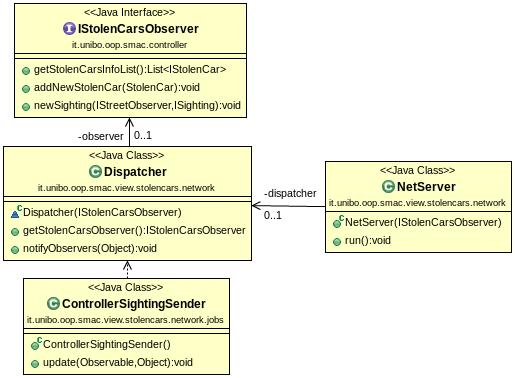
\includegraphics[width=0.48\textwidth]{images/UMLnetworkObserver}
	\caption{UML descrittivo degli obsever nel Network}
	\label{fig:UMLnetworkObserver}
      \end{center}
    \end{wrapfigure}
      Anche la Network è stata progettata per essere estesa. Per questo alla 
      ricezione dei messaggi da parte del \textit{NetServer}, questi ultimi 
verranno passati al \textit{Dispatcher} (che implementa la classe 
\textit{Observable}), il quale provvederà a richiamare tutti i Job (Observer) 
che si sono messi in ascolto. In questo modo basta aggiungere un nuovo Job che 
gestirà automaticamente i nuovi messaggi che si prevede vengano ricevuti dalla 
rete. \newline
Esempio: il job \textit{ControllerSightingSender} gestirà l'arrivo dei messaggi 
\textit{PlainSighting}. Una volta aggiunto, si occuperà di tradurre il messaggio 
dal formato di rete (come \textit{PlainSighting}), al formato compatibile con 
l'applicazione (\textit{Sighting}), e informare il controller generando un 
evento nell'osservatore della view (\textit{IStolenCarObserver}).
  
\chapter{Sviluppo}

\section{Testing}

  I punti critici dell'applicazione di cui si deve verificare il funzionamento, 
  sono 3, e per ognuno è stato adottato uno specifico metodo di test: 
  \begin{itemize}
    \item il database che si occupa della memorizzazione dei dati;
    \item il network che deve interagire con il server;
    \item la GUI che deve interagire con l'utente.
  \end{itemize}


  \subsection{Test Automatico, Model}

    Per ogni Model, abbiamo creato una serie di test che andassero a verificare 
    ogni operazione eseguibile sulla base di dati.\newline
    JUnit si è dimostrando estremamente utile anche in fase di sviluppo, 
    permettendoci di controllare che le modifiche effettuate non andassero ad 
    impattare sul risultato aspettato. Inoltre sono stati controllati non solo 
i casi in cui le funzioni avrebbero dovuto gestire i casi di successo 
(passando sempre i parametri corretti) ma anche i casi in cui 
avrebbero dovuto restituire un'eccezione, in modo da avere una copertura a 
tutto tondo dei casi d'utilizzo.


  \subsection{Test SemiAutomatico, Network}
    Volendo dare prova pratica del funzionamento dell'interaccia del Network 
    abbiamo dovuto provvedere alla creazione di un generatore di messaggi, che 
    simula il comportamento di uno Street Observer.\newline
    La verifica della simulazione verrà effettuata manualmente dall'utente, 
    controllando che all'apertura dell'applicazione vengano segnalati i 
    \textit{Sightings} sulla mappa, e nel pannello delle informazioni, i 
passaggi delle macchine. Se la GUI non dovesse visualizzare alcuna informazione, 
ovviamente questo Test dovrebbe essere ritenuto fallito.

  \subsection{Test Manuale, GUI}
    Il test delle funzionalità della GUI, in cui si sarebbe dovuto simulare il 
    comportamento dell'utente, è stato di tipo manuale. 

\section{Librerie}

  Per migliorare le condizioni di sviluppo, e per offrire funzionalità grafiche 
avanzate, ci siamo appoggiati su 5 librerie:
  \begin{itemize}
    \item \textit{slf4j} (Simple Loggin Facade for Java), per ottenere la più 
assoluta libertà nel Logging. Infatti slf4j permette di scrivere i log su 
molteplici dispositivi, dalla semplice console, a files.
    \item \textit{ormlite}, il quale offre un'interfaccia ORM (Object-Relational 
Mapping) per accedere e salvare semplicemente i dati. In particolare in questa 
versione del software, abbiamo deciso che lo store dei dati sarà effettuato in 
memoria RAM. 
Questa decisione è stata presa in particolare per non gravare sul setup 
dell'applicazione (se avessimo deciso che si doveva collegare a un database 
MySQL o Oracle, ovviamente era necessaria anche la relativa configurazione).
    \item \textit{JMapViewer}, che permette di implementare facilmente una 
schermata con mappa scorrevole e autocaricante in stile Google Maps, ma con la
ampia liberà di utilizzo che il servizio messo a dispozione da OpenStreetMap. 
Inizialmente infatti avevamo pensato di usare proprio le mappe di Google come
dichiarato nella fase iniziale del progetto, ma successivamente 
abbiamo trovato una serie di problemi: la licenza pone forti condizioni 
sull'utilizzo; la libreria non è implementata in Java nativo, ma attraverso 
un wrapper di una WebView, peggiorando così le prestazioni e le possibilità di 
utilizzo, ed è in oltre necessario inserire all'interno dell'applicazione la 
propria chiave personale di sviluppo Google per usufruire dei servizi, 
generando una potenziale divulgazione che non è auspicabile.  
    \item \textit{Netty}, una libreria per gestire il networking dalle enormi 
possibilità, la quale sta venendo sempre più utilizzata anche da colossi 
dell'informatica come Twitter, Apple ed altri (per una lista completa 
(http://goo.gl/jRb69k). \newline Il suo successo probabilmente è 
derivato dall'alta facilità d'utilizzo, la grande estendibilità e performance. 
Infatti grazie a questa libreria, che implementa un sistema ad-hoc di gestione 
delle connessioni basandosi sulla strategia NIO (Non-Blocking IO), ci permette 
di astrarci da problematiche di performance relative alla rete, concentrandoci 
solo sul message passing. 
    \item \textit{gson}, è stata utilizzata per configurare il simulatore 
degli street observer. Infatti, tramite file JSON all'interno del progetto, è 
possibile specificare, in quali punti passeranno le macchine, senza dover 
andare a specificare queste informazioni programmaticamente.
  \end{itemize} 

\section{Divisione dei compiti e metodologia di lavoro}

I primi giorni di sviluppo sono stati investiti per cercare di creare 
un'architettura UML più coerente possibile al progetto finale. Data la 
dimensione del progetto successivamente sono state fatte alcune modifiche, ma 
lasciando completamente invariata la relazione che c'era tra i 
macroblocchi.\newline
Per quanto riguarda la divisione compiti in linea generale è stata totalmente 
rispettata, tranne per la creazione dell'interfaccia della mappa che era 
stata affidata ad entrambi, ma alla fine trattandosi di un miniblocco, Bellini 
ha completato senza l'apporto di Capponi. La parte di database inoltre è 
stata creata in stretta collaborazione tra i due sviluppatori, in quanto comune 
ad entrambi, anche se legata ad aspetti differenti(salvataggio dati degli 
Osservatori/auto rubate). 
Le parti per la correzione di bugs e warnings generati dai plug-in checkStyle, 
PMD, FindBugs e qualche refactoring sono stati svolti da entrambi gli 
sviluppatori.\newline
La divisione dei compiti era:
\begin{itemize}
  \item Bellini: parte server: elaborazione dati ricevuti (controller), GUI del 
server (parte degli Osservatori), salvataggio dei dati ottenuti dai client su 
un DB (Model), interfaccia che utlizza APIs Google Maps(poi APIs del progetto 
OpenStreetMap).
  \item Capponi: parte client: invio di dati pseudo-casuali per simulazione, 
creazione di una connessione tra server e clients, gestione del database di 
auto rubate (ModelStolenCars), GUI del server (parte delle auto rubate), 
interfaccia che utlizza API Google Maps (solo Bellini), eventuale elaborazione 
del flusso di veicoli dentro e fuori dalla città (non fatta poiché fuori monte 
ore).
\end{itemize}

Come autocritica possiamo dire che la lista di compiti originariamente stilata, 
non era molto dettagliata e precisa, e ciò che non era stato scritto (come la 
creazione del Network, o la GUI per la gestione delle Stolen Cars, sviluppate 
entrambe da Capponi) può essere inteso come la diretta conseguenza della 
creazione delle altre parti del software.

  \section{Criticità}
    In una prima fase, avevamo progettato di implementare la mappa degli Street 
Observers tramite le librerie di Google Maps, pensando che fossero 
perlomeno simili a quelle della versione Android. Per nostra sfortuna, 
erano completamente diverse, e il supporto ad esse era minimo. Per questo 
motivo, abbiamo deciso di passare alla seconda scelta basata sul progetto 
OpenSource OpenStreetMap, che invece offriva un ottima libreria, che ha 
velocizzato lo sviluppo enormemente.\newline
    Un'altra question riguarda la \textit{ViewGUI}: l'idea iniziale era quella 
di renderla una classe decorabile, in modo da poter aggiungere pannelli man 
mano, come ad esempio \textit{ViewGUIStolenCars}. La problematica è venuta fuori 
quando ci siamo resi conto che non poteva essere un vero e proprio decorator, 
poiché ognuno di questi decorator avrebbero aggiunto dei metodi, che sarebbero 
dovuti essere richiamati dopo l'inizializzazione nel controller (come 
\textit{attachStolenCarsController} all'interno di \textit{ViewGUIStolenCars}). 
Per questo abbiamo preferito non ``inventarci`` un pattern ad hoc, ma lasciare 
la classe come estensione della precedente.
    
   
\chapter{Commenti finali}
  Il progetto nel complesso è stato sviluppato secondo le idee iniziali che ci 
eravamo prosti, incontrando soltanto piccole difficoltà con l'utilizzo delle 
APIs messe a disposizione da Google e con qualche difficoltà sulle librerie di 
database. Osservando il progetto nella sua interezza si può notare che il suo 
punto di forza risiede nella facilità di annettere future estensioni del 
software, senza apportare radicali cambiamenti al codice già prodotto.

  \section{Sviluppi futuri}
  Questo software non è stato sviluppato con secondi fini o scopi, ma puramente 
come attività didattica per il progetto del corso di Programmazione ad Oggetti 
a.a. 2014/2015 della facoltà di Ingegneria e Scienze Informatiche di Cesena. 
Per questo motivo non prevediamo futuri sviluppi.

\chapter{Guida Utente}
  
  Aperta la schermata si dovrà aspettare qualche secondo che il server si avvii 
e inizi a generare i Sightings. \newline
  In questa fase potrebbe accadere che l'applicazione generi un errore e si 
chiuda. 
Questo errore è dato dalla mancata inizializzazione del server network perché ha 
trovato la porta \textit{8007} occupata.
  In seguito si visualizzeranno 3 schede:
   \begin{itemize}
    \item una in cui si possono consultare le statistiche degli Street Observer.
    \item una in cui possiamo vedere la reale posizione nella mappa.
    \item una in cui possiamo gestire le macchine rubate.
   \end{itemize}
   
   N.B. Nella mappa è importante notare che il tasto usato per trascianre la 
mappa non è il sinistro, come siamo abituati tradizionalmente, ma il destro. Lo 
scroll del mouse funziona invece come di consueto come zoom per la mappa.
  \newline
  \newline
  L'ultimo pannello è quello più interattivo: si gestisce il database delle 
macchine rubate. In alto a sinistra è presente una casella di input in cui 
inserire una targa di cui si vuole fare il track. Per trovarne una valida, 
basta visualizzare l'ultima targa avvistata da un'osservatore, ed inserirla nel 
database di auto rubate. Da lì a poco si vedrà il database delle segnalazioni 
aumentare di dimensione.

\end{document}




